% !TEX root = ../../../main.tex
% 所属：第一部分：单变量分析学 / 第8章：Riemann积分
% 节：8.6 反常积分
% 正文按原文件顺序保存；由 ../chapter8.tex 调用。
\section{反常积分}
如果下列条件至少有一个满足：

1. 积分区间不是有界的闭区间，即区间为
\[
[a, +\infty),\ (-\infty, a],\ (-\infty, +\infty)
\]

2. 被积函数 \( f(x) \) 无界

我们称这样的积分为\textbf{反常积分}.

也就是说，我们需要研究两种类型的反常积分.

\begin{definition}(无限区间上的反常积分)\label{无限区间上的反常积分}
	对于反常积分
	\[
	\int_a^{+\infty} f(x)\dd x
	\]
	若对任意 \(A \ge a\)，\(f(x)\) 在 \([a,A]\) 上有界且 Riemann 可积，函数
	\[
	F(A) = \int_a^A f(x)\dd x
	\]
	若当 \(A \to +\infty\) 时，极限 \(F(A) \to I\)（其中 \(I\) 为有限数），就称反常积分
	\[
	\int_a^{+\infty} f(x)\dd x
	\]
	在 \([a,+\infty)\) 上收敛，且收敛于 \(I\)，也称 \(f(x)\) 在 \([a,+\infty)\) 上可积.此时
	\[
	\int_a^{+\infty} f(x)\dd x = I = \lim_{A \to +\infty} F(A) = \lim_{A \to +\infty} \int_a^A f(x)\dd x
	\]
	否则就称 \(f(x)\) 在 \([a,+\infty)\) 上发散.
\end{definition}
下面举一个重要的例子.

\begin{example}
	讨论区间 $[1,+\infty)$ 上的 $p$-积分
	\[
	\int_1^{+\infty} \frac{\dd x}{x^p}
	\] 的敛散性
\end{example}
\begin{solution}
	对任意 $A\geqslant1$，记
	\[
	F(A) = \int_1^A \frac{\dd x}{x^p}
	\]
	
	当 $p=1$ 时：
	\[
	F(A) = \int_1^A \frac{\dd x}{x} = \ln A
	\]
	于是
	\[
	\int_1^{+\infty} \frac{\dd x}{x} = \lim_{A \to +\infty} F(A) = +\infty
	\]
	故此时反常积分发散.
	
	当 $p \neq 1$ 时，
	\[
	F(A) = \int_1^A \frac{\dd x}{x^p} = \left. \dfrac{x^{1-p}}{1-p} \right|_1^A = \dfrac{1}{1-p} \left( \frac{1}{A^{p-1}} - 1 \right)
	\]
	
	当 $A \to +\infty$ 时：
	若 $p-1 > 0$，则 $F(A) \to \dfrac{1}{p-1}$
	;若 $p-1 < 0$，则 $F(A) \to +\infty$
	
	故对 $\displaystyle\int_1^{+\infty} \dfrac{\dd x}{x^p}$，有
	\[
	\begin{cases}
		p>1 \text{ 时，收敛} \\
		p \leq 1 \text{ 时，发散}
	\end{cases}
	\]
\end{solution}
类似地，我们可以定义 $\displaystyle\int_{-\infty}^a f(x)\dd x$，$f(x)$ 在 $[A,a]$ 上有界且 Riemann 可积，$F(A)=\displaystyle\int_A^a f(x)\dd x$.那么称 $\displaystyle\int_{-\infty}^a f(x)\dd x$ 收敛当且仅当 $\lim\limits_{A\to -\infty} F(A)$ 存在且有限.对 $\displaystyle\int_{-\infty}^{+\infty} f(x)\dd x$，取 $a\in(-\infty,+\infty)$，有
\[
\int_{-\infty}^{+\infty} f(x)\dd x = \int_a^{+\infty} f(x)\dd x + \int_{-\infty}^a f(x)\dd x
\]
分别讨论即可.

必需强调的是
\[
\lim_{A\to\infty} \int_{-A}^A f(x)\dd x \neq \int_{-\infty}^{+\infty} f(x)\dd x
\]
\begin{example}
	\[
	\int_{-A}^A \sin x \dd x  = 0 \quad \text{故} \quad \lim_{A \to +\infty} \int_{-A}^A \sin x \dd x = 0
	\]
	而
	\[
	\int_0^{+\infty} \sin x \dd x = \lim_{A \to +\infty} \int_0^A \sin x \dd x = \lim_{A \to +\infty} \left. (1 - \cos x) \right|_0^A \quad \text{发散}
	\]
	同理
	\[
	\int_{-\infty}^0 \sin x \, \dd x = \lim_{A \to -\infty} \int_A^0 \sin x \, \dd x = \lim_{A \to -\infty} \left. (1 - \cos x) \right|_A^0 \quad \text{发散}
	\]
	
\end{example}


但我们可以定义这样一种积分，作为在 $(-\infty,+\infty)$ 上的推广.
\begin{definition}
	若
	\[
	\lim_{A \to \infty} \int_{-A}^A f(x) \dd x = \lim_{A \to \infty} \left( F(A) - F(-A) \right)
	\]
	收敛，则称该极限值为 $\displaystyle\int_{-\infty}^{+\infty} f(x)\dd x$ 的 Cauchy主值，记为
	\[
	(\text{cpv}) \int_{-\infty}^{+\infty} f(x) \, \dd x
	\]
	
	当 $\displaystyle\int_{-\infty}^{+\infty} f(x) \dd x$ 收敛时，显然有
	\[
	(\text{cpv}) \int_{-\infty}^{+\infty} f(x) \dd x = \int_{-\infty}^{+\infty} f(x) \dd x
	\]
	但是 $\displaystyle\int_{-\infty}^{+\infty} f(x) \dd x$ 发散时，它的 Cauchy 主值可以存在.
	
\end{definition}
设函数 $f(x)$ 在 $[a,b]$ 上无界，若存在 $c \in [a,b]$，使得 $f(x)$ 在 $c$ 的任一邻域内无界，则称 $c$ 为 $f(x)$ 的一个奇点.设 $[a,b]$ 上有有限个奇点 $c_1 < c_2 < \dots < c_n\in [a,b]$.

以 $m=2$，即 $a \le c_1 < c_2 \le b$ 为例，有
\[
\int_a^b f(x)\dd x = \int_a^{c_1} f(x)\dd x + \int_{c_1}^{d_1} f(x)\dd x + \int_{d_1}^{c_2} f(x)\dd x + \int_{c_2}^b f(x)\dd x
\]
上式右端的所有反常积分都收敛，当且仅当 $\displaystyle\int_a^b f(x)\dd x$ 收敛.因此，我们只需考虑在端点处有唯一奇点的情况.
\begin{definition}(有限闭区间上的无界函数的反常积分)\label{有限闭区间上的无界函数的反常积分}
	
	
	设 $f(x)$ 在 $[a,b]$ 上有唯一奇点，且为右端点 $b$.对任意 $\eta>0$，$b-\eta \in (a,b)$，$f(x)$ 在 $[a,b-\eta]$ 上有界且 Riemann 可积，定义
	\[
	F(\eta) = \int_a^{b-\eta} f(x)\dd x
	\]
	若极限 $\lim\limits_{\eta \to 0^+} F(\eta)$ 存在且有限，记为 $I$，则称反常积分 $\displaystyle\int_a^b f(x)\dd x$ 收敛于 $I$，即
	\[
	\int_a^b f(x)\dd x = \lim_{\eta \to 0^+} \int_a^{b-\eta} f(x)\dd x
	\]
\end{definition}
\begin{example}
	$(0,1]$ 上的 $p$-积分
	
	讨论反常积分
	\[
	\int_0^1 \frac{\dd x}{x^p}
	\]
	的敛散性.
\end{example}
\begin{solution}
	当 $p \neq 1$ 时，
	\[
	\int_0^1 \frac{\dd x}{x^p} = \lim_{\eta \to 0^+} \int_\eta^1 \frac{dx}{x^p}
	= \lim_{\eta \to 0^+} \left( \frac{1}{1-p} \right) \left( 1 - \eta^{1-p} \right)
	=
	\begin{cases}
		+\infty, & p>1 \\
		\dfrac{1}{1-p}, & p<1
	\end{cases}
	\]
	
	当 $p=1$ 时，
	\[
	\int_0^1 \frac{\dd x}{x} =\ln x |_0^1 = +\infty
	\]
	
	故
	\[
	\begin{cases}
		p \ge 1, & \text{发散} \\
		p < 1, & \text{收敛}
	\end{cases}
	\]
\end{solution}

\ref{无限区间上的反常积分} 与\ref{有限闭区间上的无界函数的反常积分} 的两类反常积分可以互相转化.

对
\[
\int_a^{+\infty} f(x) \dd x
\]
不妨设 \(a>0\)，令 \(x=\dfrac{1}{t}\)，则 \(\dd x=-\dfrac{1}{t^2}\dd t\)，于是
\[
\int_a^{+\infty} f(x) \dd x = \int_0^{1/a} \frac{1}{t^2} f\left( \frac{1}{t} \right) \dd t
\]

对
\[
\int_a^b f(x) \dd x
\] 
令 \(t=\dfrac{1}{b-x}\)，则 \(x=b-\dfrac{1}{t}\)，\(dx=\dfrac{1}{t^2}\dd t\)，于是
\[
\int_a^b f(x) \dd x = \int_{\tfrac{1}{b-a}}^{+\infty} \frac{1}{t^2} f\left( b-\frac{1}{t} \right) \dd t
\]

若 \(\displaystyle\int_a^{+\infty} f(x)dx\) 收敛，不能保证 \(\lim\limits_{x\to+\infty} f(x)=0\)，甚至不能保证 \(f(x)\) 在 \([a,+\infty)\) 上有界.
\begin{example}
	设 $f(x)$ 在 $[1,+\infty)$ 按以下方式定义：
	\[
	f(x) =
	\begin{cases}
		n+1, & x \in \left[ n, n+\dfrac{1}{n(n+1)^2} \right] \\
		0, & x \in \left( n+\dfrac{1}{n(n+1)^2}, n+1 \right)
	\end{cases}
	\quad n=1,2,\dots
	\]
	下证 $\displaystyle\int_1^{+\infty} f(x)\dd x$ 收敛.
\end{example}
\begin{center}
	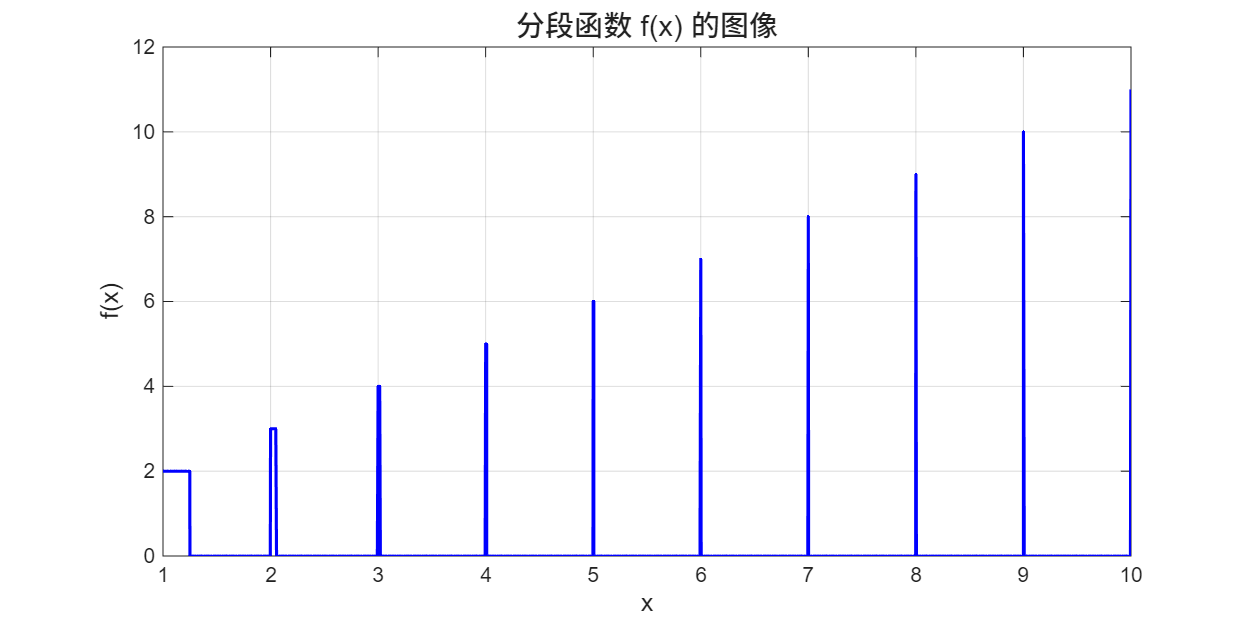
\includegraphics[width=0.7\linewidth]{figure/C7/untitled}
\end{center}

\begin{proof}
	对任意 $A>1$，取 $n \in \mathbb{N}$，使 $A \in [n,n+1)$.由 $f(x) \ge 0$，有
	\[
	\int_1^n f(x)\dd x \le \int_1^A f(x)\dd x \le \int_1^{n+1} f(x)\dd x
	\]
	
	当 $n \to +\infty$ 时，
	\[
	\begin{aligned}
		\lim_{n \to \infty} \int_1^n f(x)\dd x &= \lim_{n \to \infty} \left[ \int_1^2 f(x)\dd x + \dots + \int_{n-1}^n f(x)\dd x \right] \\
		&= \lim_{n \to \infty} \left[ \frac{1}{1 \cdot 2} + \frac{1}{2 \cdot 3} + \dots + \frac{1}{(n-1)n} \right] \\
		&= \lim_{n \to \infty} \left( 1 - \frac{1}{2} + \frac{1}{2} - \frac{1}{3} + \dots + \frac{1}{n-1} - \frac{1}{n} \right) \\
		&= \lim_{n \to \infty} \left( 1 - \frac{1}{n} \right) = 1
	\end{aligned}
	\]
	
	同理
	\[
	\lim_{n \to \infty} \int_1^{n+1} f(x)\dd x = 1
	\]
	由夹逼性
	\[
	\int_1^{+\infty} f(x)\dd x = 1
	\]
	
	
\end{proof} 
类似的方式，即使 $f(x)$ 在 $[a,+\infty)$ 连续（$n$ 次可微），也可以构造出使 $\displaystyle\int_a^{+\infty} f(x)dx$ 收敛而 $f(x)$ 在 $[a,+\infty)$ 无界的例子.

对反常积分的计算，我们可以形式上认为
\[
\int_a^{+\infty} f(x)\dd x = \lim_{A \to +\infty} F(A) - F(a)
\]

